\pgfdeclarelayer{bg}    % declare background layer
\pgfsetlayers{bg,main}  % set the order of the layers (main is the standard layer)

\tikzset{
every node/.style={draw,text width=2cm},
style1/.style= {rectangle, thin, align=center, fill=gray!20, text width=5cm},
style2/.style= {rectangle, thin, align=left,yshift=-2cm, text width=4cm}
}



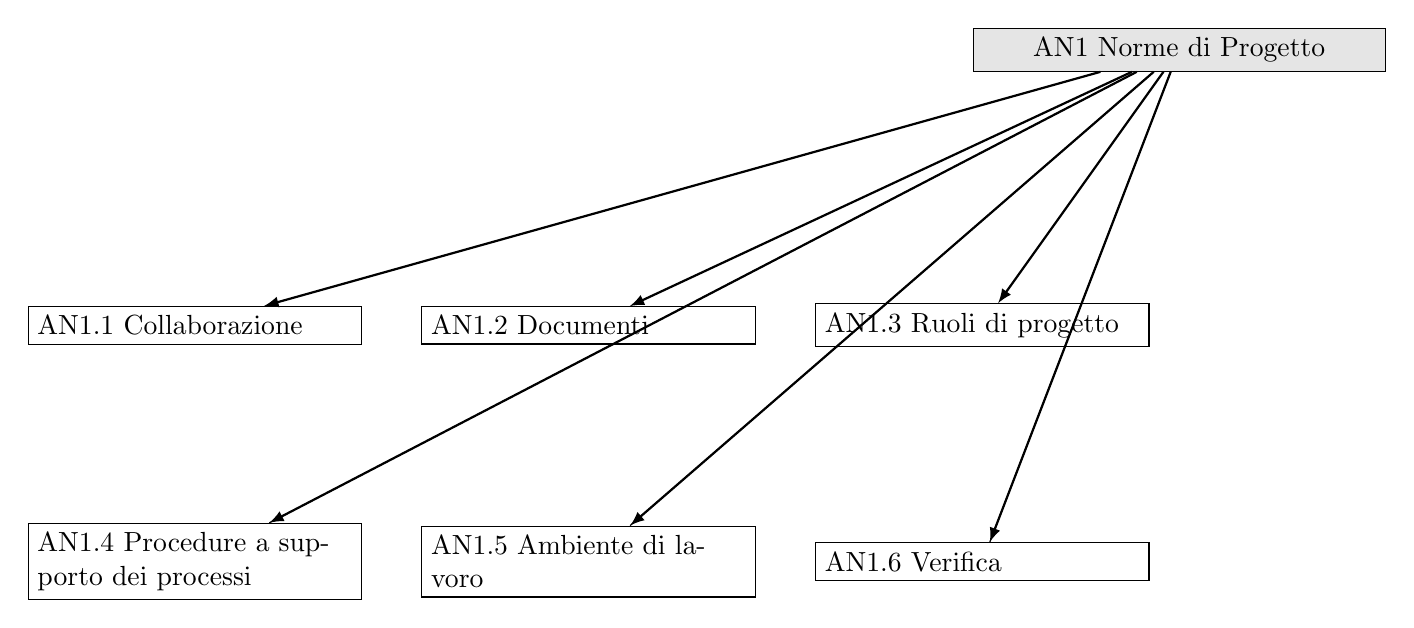
\begin{tikzpicture}[
remember picture,
level 1/.style={sibling distance=50mm},
edge from parent/.style={->,draw,thick},
>=latex]

% the initial tree ("root" and "text nodes")
\node[style1] (1) {AN1 Norme di Progetto}
child {node[style2] (c1) {AN1.1 Collaborazione}}
child {node[style2] (c2) {AN1.2 Documenti}}
child {node[style2] (c3) {AN1.3 Ruoli di progetto}}
child {node[style2, below of=c1] (c4) {AN1.4 Procedure a supporto dei processi}}
child {node[style2, below of=c2] (c5) {AN1.5 Ambiente di lavoro }}
child {node[style2, below of=c3] (c6) {AN1.6 Verifica}};

 \begin{pgfonlayer}{bg}
    \path[every node/.style={font=\sffamily\small}]
    (1) edge (c4)
        edge (c5)
        edge (c6);
  \end{pgfonlayer}


\end{tikzpicture}



